\section{Description}
This module is responsible for storing users and patterns, communicating with
the client and running the Siddhi engine. Furthermore, it is the endpoint where
all sensors have to sent their data in order to be processed by the Siddhi engine.
The server primarily consists of
\begin{itemize}
    \item controllers - to manage the stored data
    \item handlers - to coordinate network communication
    \item the Siddhi engine - to process events and detect patterns
    \item loggers - to keep a log of all events, errors and actions occuring
    \item command-line-interface (cli) - to provide the admin console
\end{itemize}

\section{Overview}
\FloatBarrier
\begin{figure}
    \centering
    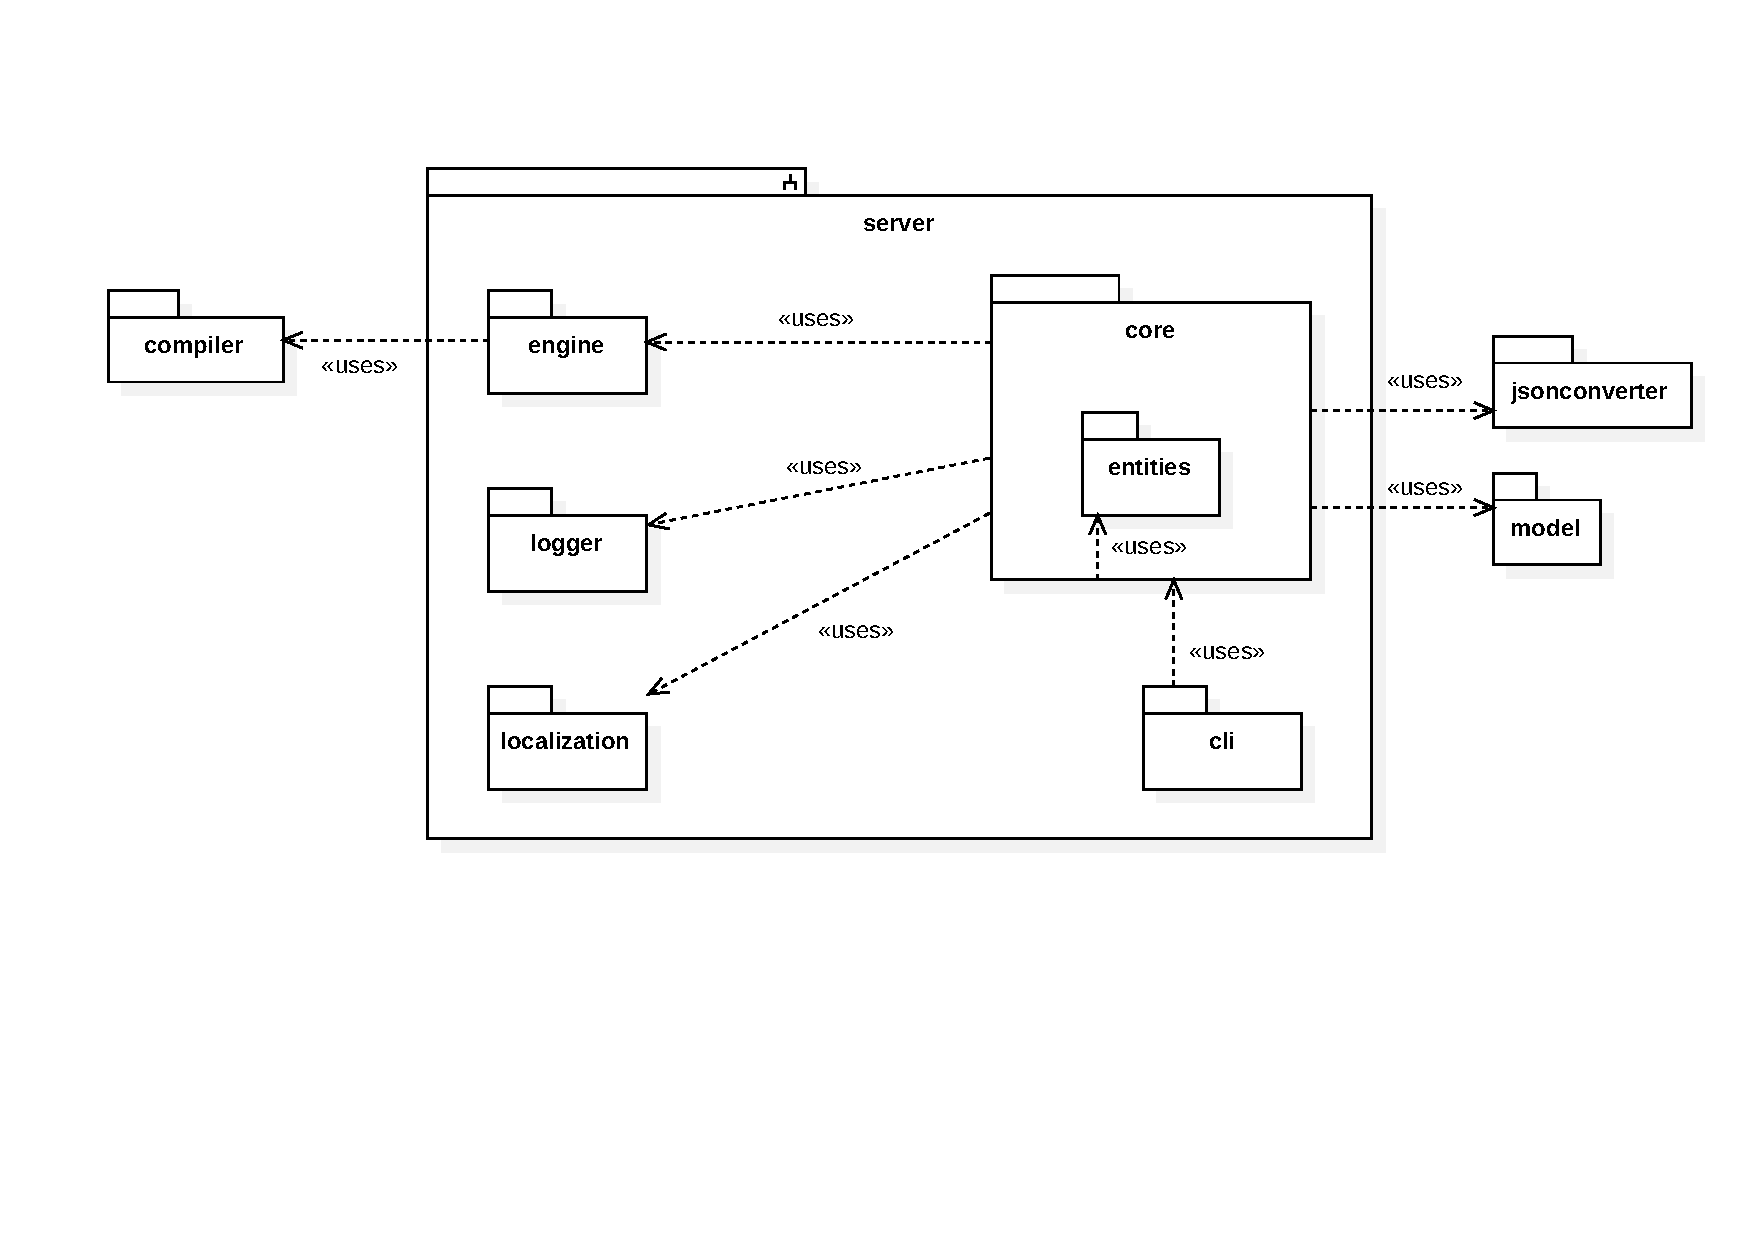
\includegraphics[width=\textwidth]{../module_res/server-package.pdf}
    \caption{UML package Diagram of the server module with uses-relations.
    (Uses-relations between other modules were omitted).
    \label{fig:server-package}}
\end{figure}
\FloatBarrier


\section{Design Patterns}
The important goal of delivering most-possible independence from other libraries
involved several \emph{wrappers} for the core tasks of the server.
For handling incoming HTTP requests (e.g. from the client or sensors), there is
the \texttt{IRequestHandler} interface. Our specific implementation uses
the \enquote{Spark} library which is wrapped in the \texttt{SparkServer} class.
The socket actions used in patterns need a socket server whose functionality is
defined in the \texttt{ISocketHandler} interface. Our implementation uses the
\enquote{Webbit} library which is wrapped in the \texttt{WebbitSocket} class.
This approach was also used for database interaction (\texttt{IDatabaseConnector}
realized by \texttt{MongoDBConnector} wrapping the \enquote{MongoDB Java driver}) as well as
the CEP engine (\texttt{IEngine} realized by \texttt{SiddhiEngine} wrapping the
\enquote{WSO2 Siddhi} library). If we change our library decisions at a later state,
it is only necessary to create one new wrapper class realizing the desired interface.

To be able to handle commands and routes flexbile, they are organized using
the \emph{commando} pattern. For example, a \texttt{Command} can be passed to a
method and executed without any need to know what the command does. \\
All commands share the \emph{template method} \texttt{handle(...)} which
determines whether the user input starts with the keyword of the command
(this step is common for all commands). If so, it calls the abstract method
\texttt{execute(...)} which needs to be overridden with the actual implementation
of the command.

The situation of several server instances using different logging mechanisms
led to a \emph{strategy} pattern. The \texttt{ILogger} interface defines
various logging methods. The specific \enquote{strategies} in our case are a
\texttt{ConsoleLogger} (logs to a console), \texttt{FileLogger} (logs to a file)
and a \texttt{MultiLogger} (compound of multiple loggers). Latter makes use
of the \emph{composite} pattern and therefore, a \texttt{MultiLogger} can be used
like any other logger or even nested into another \texttt{MultiLogger}.

Furthermore, the operating part of the server is separated from the command-line-interface
and therefore follows the principles of the \emph{model-view-controller} pattern.
The model is separated as well due to its encapsulation in an external module.
This approach allows us to transition smoothly from the command-line-interface
to a graphical one.


\section{Class Diagram}
The following UML class diagram (\autoref{fig:server-class}) specifies all
classes, interfaces, public methods and attributes of the server module.

\FloatBarrier
\begin{figure}[h]
    \centering
    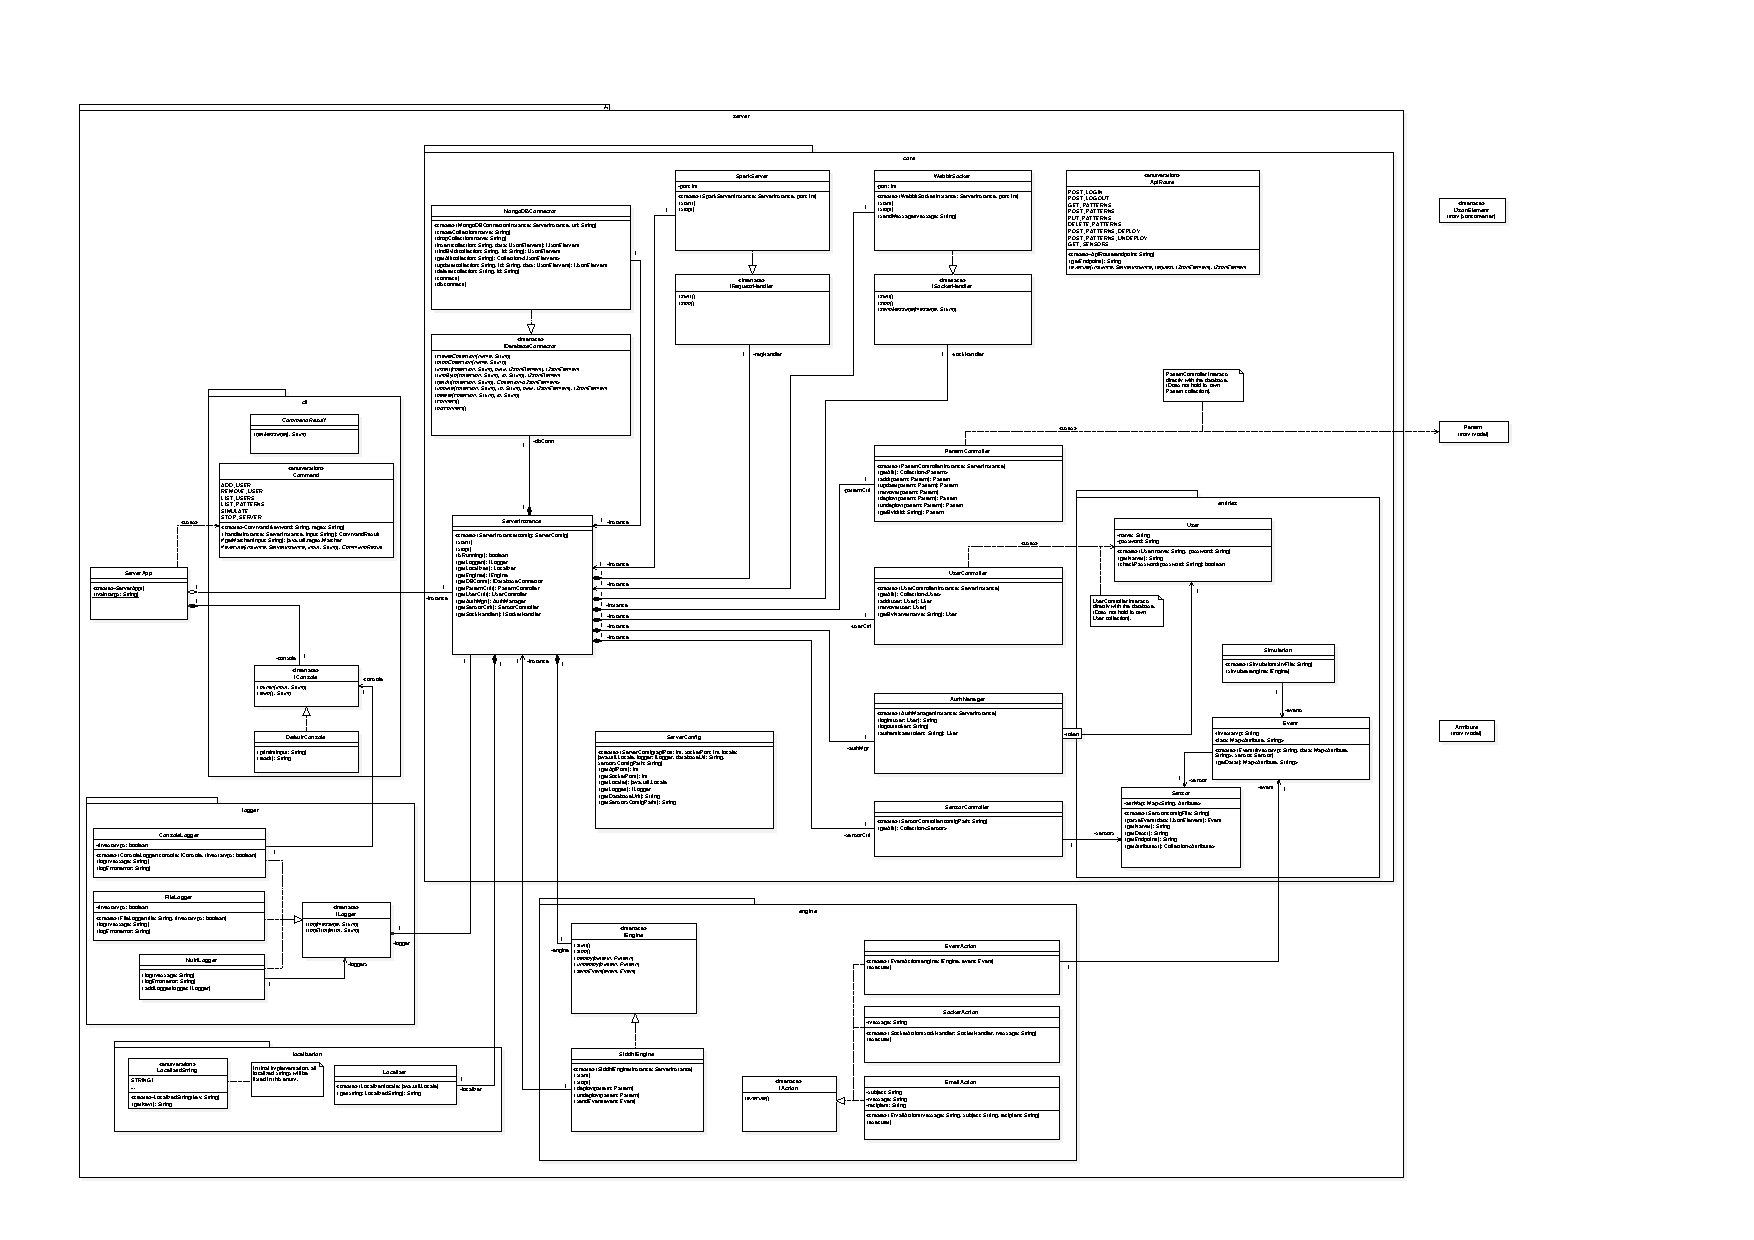
\includegraphics[width=\textwidth]{../module_res/server-class.pdf}
    \caption{Class Diagram of the server module.
    \label{fig:server-class}}
\end{figure}
\FloatBarrier


\section{Sequence Diagrams}
The following UML sequence diagrams specify the communication between classes
within this module for typcial use cases like
\enquote{Add new user} (\autoref{fig:server-sd-addusercmd}),
\enquote{Deploy pattern} (\autoref{fig:server-sd-deploypatternroute}) and
\enquote{Receive event from sensor} (\autoref{fig:server-sd-sendevent}).
\emph{(Notice: Logging operations were omitted for clarity).}

\FloatBarrier
\begin{figure}[h]
    \centering
    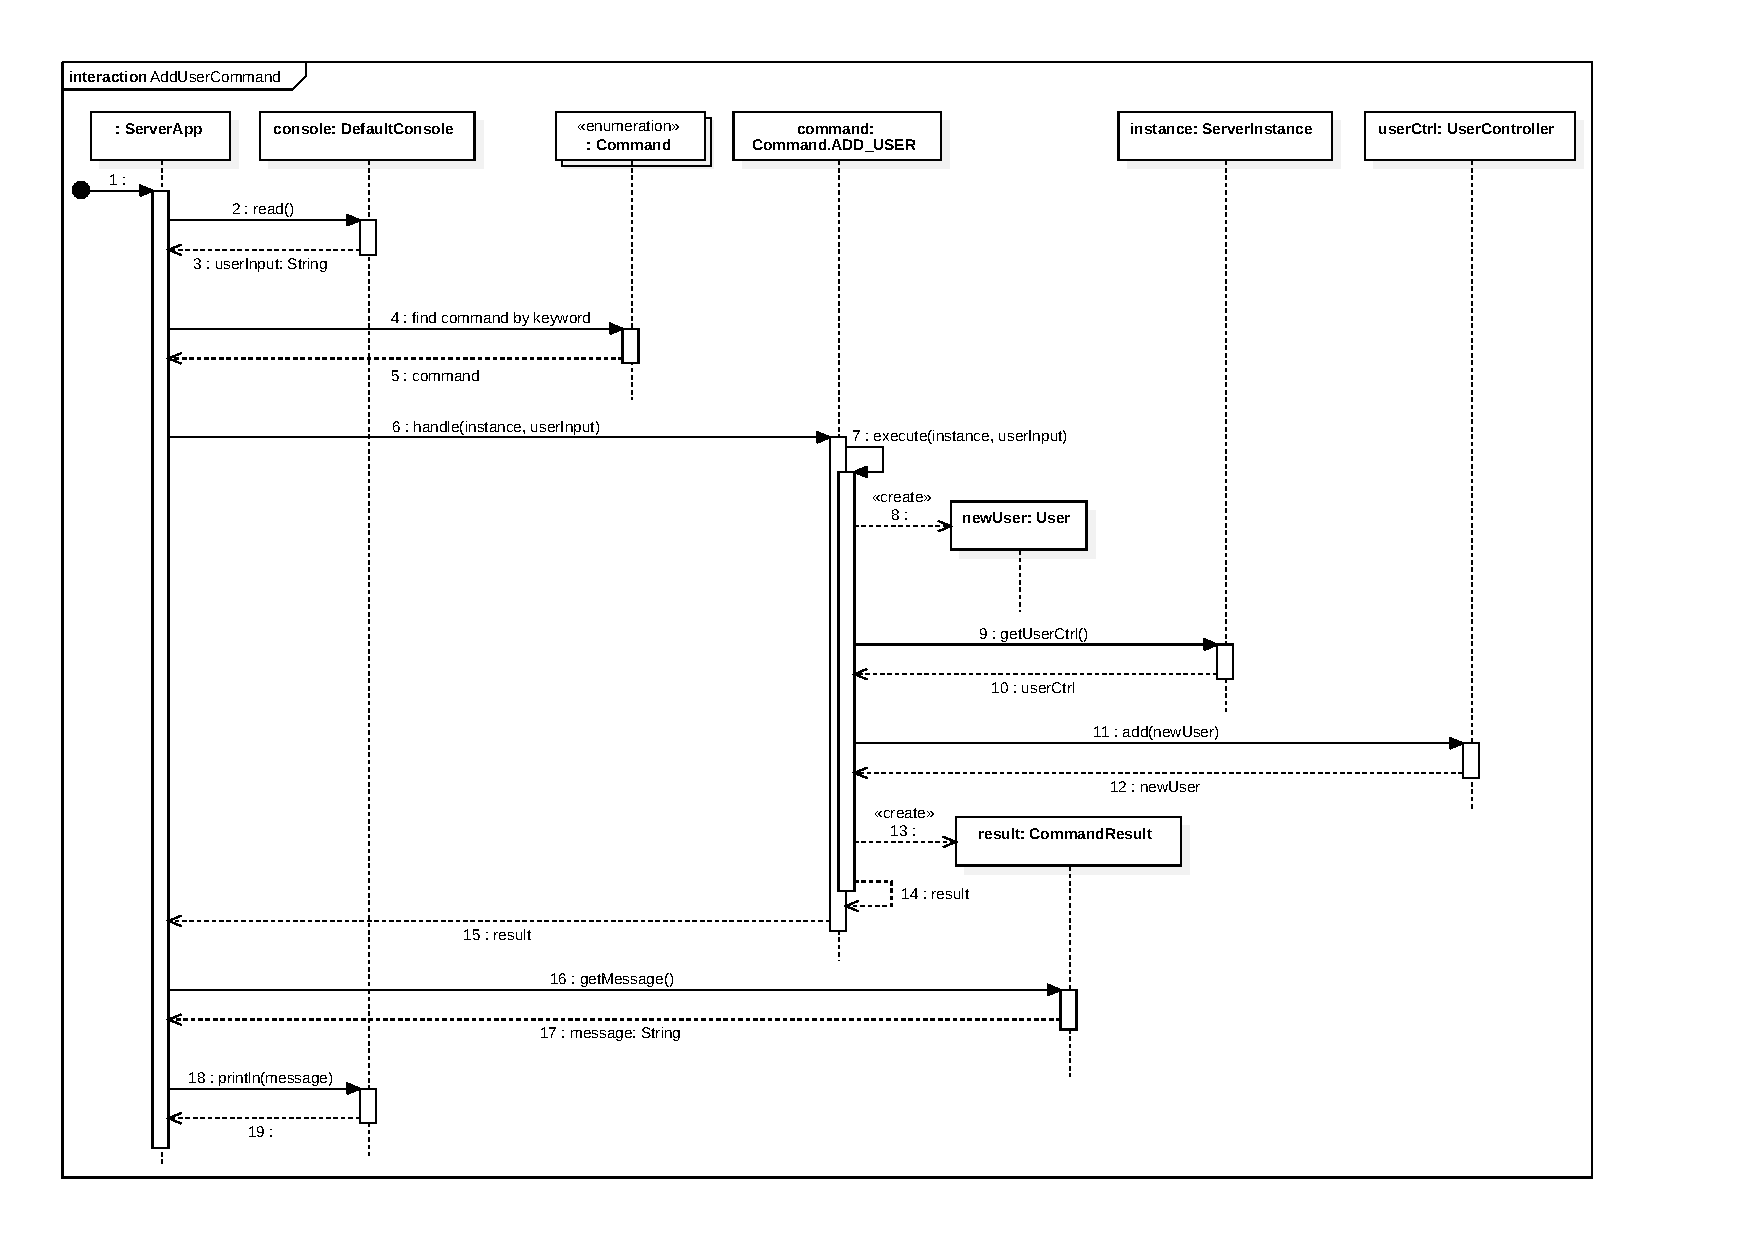
\includegraphics[width=\textwidth]{../module_res/server-sd-addusercmd.pdf}
    \caption{Sequence Diagram:
        An admin adds a new user by executing the corresponding command in the
        admin console.
    \label{fig:server-sd-addusercmd}}
\end{figure}

\begin{figure}[h]
    \centering
    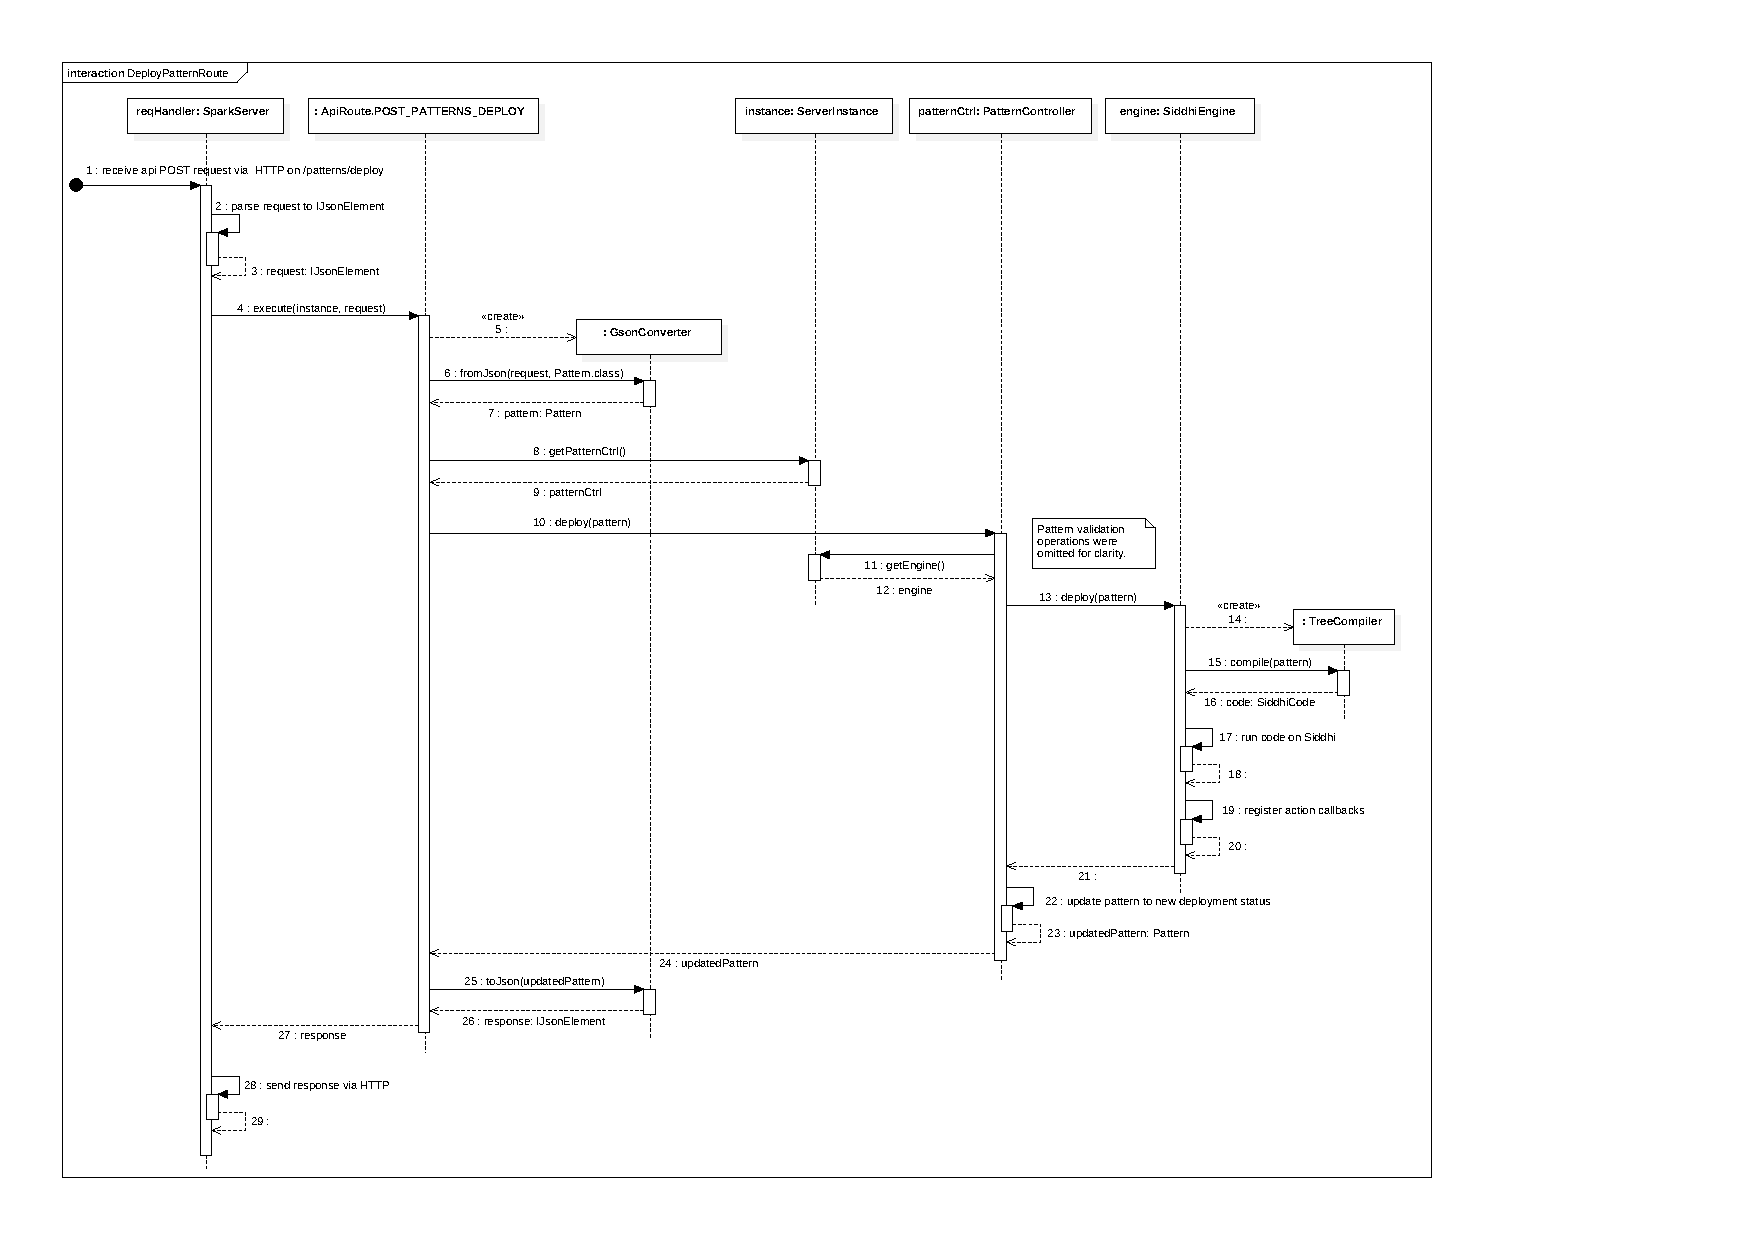
\includegraphics[width=\textwidth]{../module_res/server-sd-deploypatternroute.pdf}
    \caption{Sequence Diagram:
        The server receives an request (e.g. from a client) to deploy a pattern
        to the Siddhi engine.
    \label{fig:server-sd-deploypatternroute}}
\end{figure}

\begin{figure}[h]
    \centering
    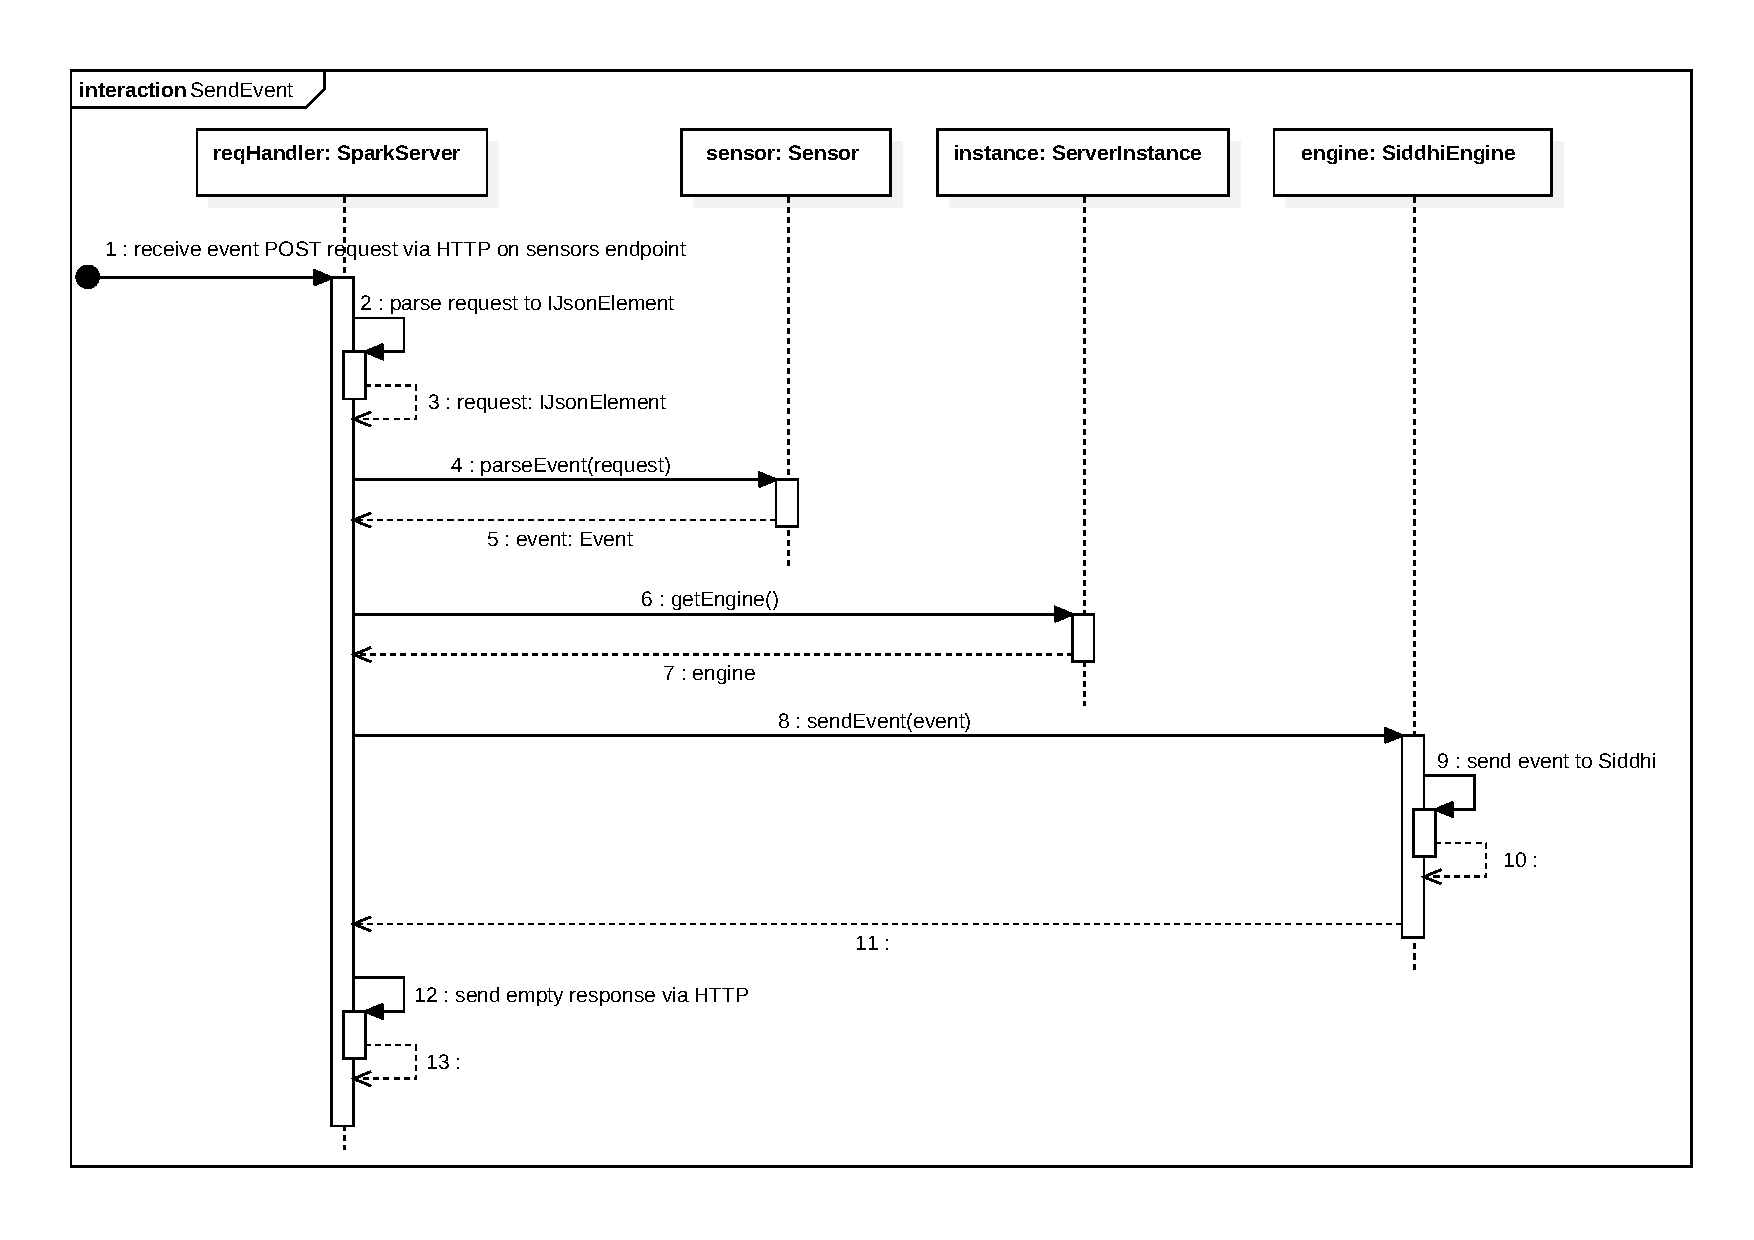
\includegraphics[width=\textwidth]{../module_res/server-sd-sendevent.pdf}
    \caption{Sequence Diagram:
        The server receives an event from a sensor and passes it to the Siddhi
        engine.
    \label{fig:server-sd-sendevent}}
\end{figure}
\FloatBarrier


\section{Activity Diagram}
The following UML activity diagram specifies the procedure runned during the
\enquote{Server startup} (\autoref{fig:server-act-start}).

\FloatBarrier
\begin{figure}[h]
    \centering
    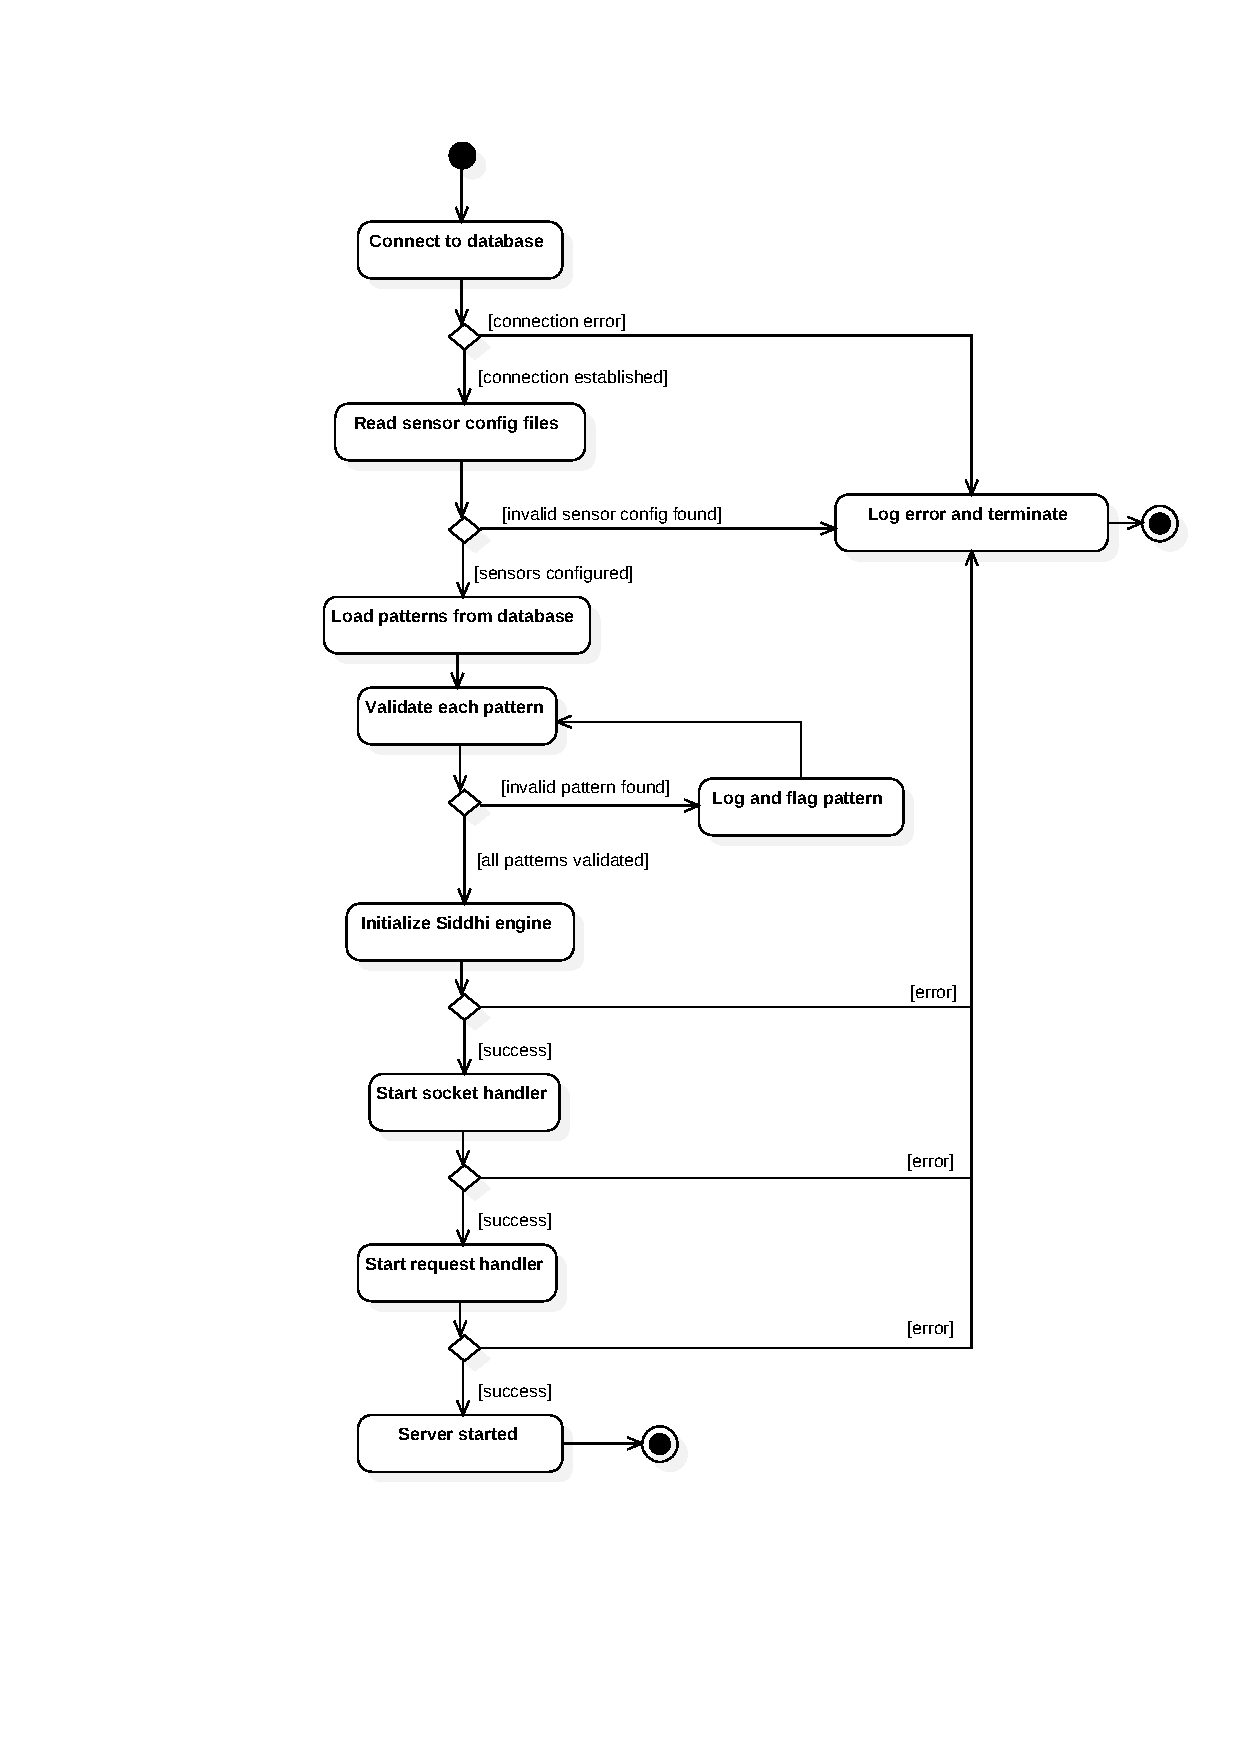
\includegraphics[width=0.7\textwidth]{../module_res/server-act-start.pdf}
    \caption{Activity Diagram:
        Actions happening after invoking the main method till the server is
        fully initialized and started.
    \label{fig:server-act-start}}
\end{figure}
\FloatBarrier
